%%%%%%%%%%%%%%%%%%%%%%%%%%%%%%%%%%%%%%%%%
% Beamer Presentation
% LaTeX Template
% Version 1.0 (10/11/12)
%
% This template has been downloaded from:
% http://www.LaTeXTemplates.com
%
% License:
% CC BY-NC-SA 3.0 (http://creativecommons.org/licenses/by-nc-sa/3.0/)
%
%%%%%%%%%%%%%%%%%%%%%%%%%%%%%%%%%%%%%%%%%

%----------------------------------------------------------------------------------------
%	PACKAGES AND THEMES
%----------------------------------------------------------------------------------------

\documentclass{beamer}
\graphicspath{{Figures/}}
\usepackage[utf8]{inputenc}  % Para codificación de texto UTF8.
\usepackage[spanish]{babel}  % Para escritura en castellano.
\usepackage{xcolor}
\usepackage{subfigure}  % Para manejo de subfiguras.
\usepackage{graphicx}
\usefonttheme[onlymath]{serif}  
\mode<presentation> {

% The Beamer class comes with a number of default slide themes
% which change the colors and layouts of slides. Below this is a list
% of all the themes, uncomment each in turn to see what they look like.

%\usetheme{default}
%\usetheme{AnnArbor}
%\usetheme{Antibes}
%\usetheme{Bergen}
%\usetheme{Berkeley}
%\usetheme{Berlin}
%\usetheme{Boadilla}
%\usetheme{CambridgeUS}
%\usetheme{Copenhagen}
%\usetheme{Darmstadt}
%\usetheme{Dresden}
%\usetheme{Frankfurt}
%\usetheme{Goettingen}
%\usetheme{Hannover}
%\usetheme{Ilmenau}
%\usetheme{JuanLesPins}
%\usetheme{Luebeck}
\usetheme{Madrid}
%\usetheme{Malmoe}
%\usetheme{Marburg}
%\usetheme{Montpellier}
%\usetheme{PaloAlto}
%\usetheme{Pittsburgh}
%\usetheme{Rochester}
%\usetheme{Singapore}
%\usetheme{Szeged}
%\usetheme{Warsaw}

% As well as themes, the Beamer class has a number of color themes
% for any slide theme. Uncomment each of these in turn to see how it
% changes the colors of your current slide theme.

%\usecolortheme{albatross}
%\usecolortheme{beaver}
%\usecolortheme{beetle}
%\usecolortheme{crane}
%\usecolortheme{dolphin}
%\usecolortheme{dove}
%\usecolortheme{fly}
%\usecolortheme{lily}
%\usecolortheme{orchid}
%\usecolortheme{rose}
%\usecolortheme{seagull}
%\usecolortheme{seahorse}
%\usecolortheme{whale}
%\usecolortheme{wolverine}

%\setbeamertemplate{footline} % To remove the footer line in all slides uncomment this line
%\setbeamertemplate{footline}[page number] % To replace the footer line in all slides with a simple slide count uncomment this line

\setbeamertemplate{navigation symbols}{} % To remove the navigation symbols from the bottom of all slides uncomment this line
}

\usepackage{graphicx} % Allows including images
\usepackage{booktabs} % Allows the use of \toprule, \midrule and \bottomrule in tables
\renewcommand{\vec}[1]{\boldsymbol{#1}}
%----------------------------------------------------------------------------------------
%	TITLE PAGE
%----------------------------------------------------------------------------------------

\title[Tesis de grado]{Estudio de estructuras de banda prohibida electromagnética (EBG) para la reducción de acoplamiento mutuo entre antenas \textit{microstrip}} % The short title appears at the bottom of every slide, the full title is only on the title page

\author{Federico Luna} % Your name
\institute[] % Your institution as it will appear on the bottom of every slide, may be shorthand to save space
{
Facultad de Ingeniería,\\
Universidad de Buenos Aires \\ % Your institution for the title page
\medskip
\textit{fluna@fi.uba.ar}\\
\medskip % Your email address
Tutores: Dr. Ing. W. Gustavo Fano y Mg. Ing. Silvina Boggi
}
\date{} % Date, can be changed to a custom date

\begin{document}

	\begin{frame}
		\titlepage % Print the title page as the first slide
	\end{frame}

\begin{frame}
\frametitle{Resumen} % Table of contents slide, comment this block out to remove it
\tableofcontents[hideallsubsections] % Throughout your presentation, if you choose to use \section{} and \subsection{} commands, these will automatically be printed on this slide as an overview of your presentation
\end{frame}

%----------------------------------------------------------------------------------------
%	PRESENTATION SLIDES
%----------------------------------------------------------------------------------------

%------------------------------------------------
\section{Presentación del problema} % Sections can be created in order to organize your presentation into discrete blocks, all sections and subsections are automatically printed in the table of contents as an overview of the talk
%------------------------------------------------
		\begin{frame}
			\frametitle{Objetivo}
			
			\begin{itemize}
				\item Propagación de ondas de superficie.
				\item Estructuras periódicas.
				\item Comportamiento de EBGs uniplanares.
				\item Modelo circuital equivalente de una celda unitaria.
				\item Programa de simulación en el dominio del tiempo.
				\item Introducción al uso de EBGs en antenas.
			\end{itemize}
		\end{frame}
	
		\begin{frame}
		\frametitle{Reseña histórica}
		\begin{itemize}
			\item 1873: \textbf{Maxwell}. Bases de teoría electromagnética clásica.\\
			\item 1885-1887: \textbf{Heaviside}. Simplificación de expresiones: Notación vectorial. \\
			\item 1886-1891: \textbf{Hertz}. Validación de teoría de ondas electromagnéticas. Primer antena dipolo y parabólica.
			\item 1897: \textbf{Rayleigh}. Propagación de ondas en guías metálicas.
			\item 1926: \textbf{Yagi-Uda}. Conjunto de antenas, fase fija.
			\item 1938-1945: Antenas de fase variable.
			\item 1953: \textbf{Deschamps}. Antenas \textit{microstrip}.
			\item 1970': Uso en aplicaciones prácticas. Solución a problemas de dispersión y modos indeseados.
			% Sustratos con bajas tangentes de pérdida. Mejora en fotolitografía. Optimización de modelos teóricos, simulaciones numéricas. Simplificación constructiva, más barato.
		\end{itemize}
		\end{frame}
	
		\begin{frame}
		\frametitle{Ventajas de las estructuras \textit{microstrip}}
		
		\begin{columns}[c] % The "c" option specifies centered vertical alignment while the "t" option is used for top vertical alignment
			
			\column{.50\textwidth} % Left column and width
			\begin{figure}[h]
				\centering
				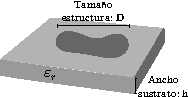
\includegraphics[width=1\textwidth]{Presentacion/microstrip_general.pdf}
			\end{figure}
			
			\column{.45\textwidth} % Right column and width
			\begin{itemize}
				\item Bajo costo.
				\item Bajo peso.
				\item Construcción sencilla (fotolitografía).
				\item Cómodas para implantación de componentes discretos.
				\item Alto Q (resonantes).
			\end{itemize}
		
		\end{columns}
	
	\vspace{25pt}
	
	\centering Aplicaciones: filtros microondas, acopladores direccionales, transformadores de impedancia, planos de tierra y redes de distribución de circuitos impresos.
		
	\end{frame}
		
		\begin{frame}
		\frametitle{Problemas de las estructuras \textit{microstrip}}
			\centering El tamaño de las antenas y estructuras \textit{microstrip} depende de la permitividad dieléctrica del sustrato y de la longitud de onda de trabajo. \\
			\begin{columns}[c] % The "c" option specifies centered vertical alignment while the "t" option is used for top vertical alignment
				
				\column{.38\textwidth} % Left column and width
				
				\begin{itemize}
					\item $\downarrow D \Rightarrow \uparrow \epsilon_r,$ {\color{red}$\uparrow$ SW}.
					\item $\uparrow \epsilon_r \Rightarrow \uparrow Q, \downarrow$ BW.
					\item $\downarrow Q \Rightarrow \uparrow h$.
					\item $\uparrow h \Rightarrow ${\color{red}$\uparrow$ SW}, $\uparrow$ modos.
				\end{itemize}
				\vspace{5pt}
				Las ondas de superficie:
				\begin{itemize}
					\item $\downarrow$ potencia radiada.
					\item {\color{red}$\uparrow$ acoplamiento.}
					\item Diagrama de radiación: \\$\uparrow$ lóbulos secundarios. %Por discontinuidades
				\end{itemize}
				
				
				\column{.60\textwidth} % Right column and width
				\begin{figure}[h]
					\centering
					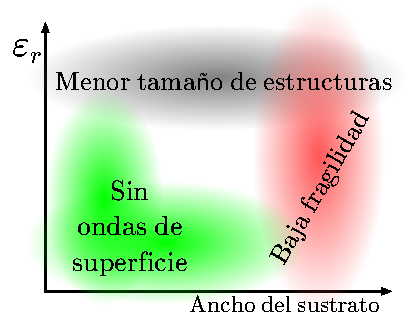
\includegraphics[width=1\textwidth]{Presentacion/problema_microstrip.pdf}
				\end{figure}
				
			\end{columns}
			\vspace{9pt}
			\centering {\footnotesize SW: Ondas de superficie. BW: Ancho de banda. $D$: Tamaño de la estructura. $h$: Ancho del sustrato.}
		\end{frame}
		
		
		% Acá la idea es comentar que en general uno busca disminuir el tamaño. Eempezando de la esquina inferior derecha, uno tiene una estructura grande y fuerte. La quiere achicar, sale de la zona verde, hay mas ondas de superficie, y para bajar esas ondas no queda otra que bajar el ancho del sustrato, generando mayor fragilidad estructural. Modos indeseados.
		\begin{frame}
		\frametitle{Soluciones propuestas en la literatura}
		
		\begin{itemize}
			\item Separación del plano de tierra de las estructuras.
			\item Modificar la altura o la permitividad del sustrato a corta distancia.
			\item Estructuras periódicas: EBG, DGS.
		\end{itemize}
		
		\begin{figure}[H]
			\centering 
			\subfigure{
				\label{fig:sustrato-antena-ebg}
				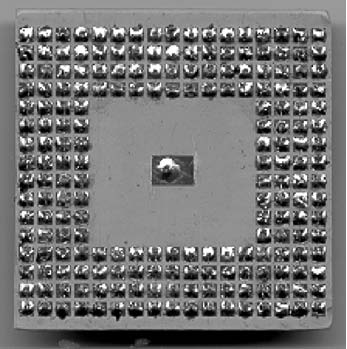
\includegraphics[width=0.40\textwidth]{Aplicacion/foto-ebg-alrededor-antena.pdf}}
			\hspace{10pt}
			\subfigure{
				\label{fig:escalon-sustrato}
				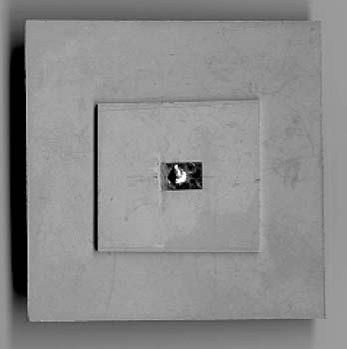
\includegraphics[width=0.40\textwidth]{Aplicacion/foto-escalon-alrededor-antena.pdf}}
		\end{figure}
		\tiny{F. Yang e Y. Rahmat-Samii, Electromagnetic Band Gap Structures in Antenna Engineering, Cambridge University Press, 2009.}
		\end{frame}

\section{Conceptos básicos de electromagnetismo}
	
	
	\begin{frame}
		\frametitle{Conceptos básicos de electromagnetismo}
		\tableofcontents[currentsection,hideothersubsections]
	\end{frame}
	
	\subsection{Ecuaciones de Maxwell} % A subsection can be created just before a set of slides with a common theme to further break down your presentation into chunks
	
		\begin{frame}
		\frametitle{Ecuaciones de Maxwell}
		
		\begin{align*}
		\left.\begin{array}{rr@{\mskip\thickmuskip}l}
		\text{Faraday} &\nabla \times \vec{E} & = -\frac{\partial \vec{B}}{\partial t} - \vec{M}\\
		\text{Ampère} &\nabla \times \vec{H} & = \frac{\partial \vec{D}}{\partial t} + \vec{J} \\
		\text{Gauss} &\nabla \cdot \vec{D} & = \rho \\
		\text{Gauss} & \nabla \cdot \vec{B} & = 0
		\end{array} \right\}
		\quad \implies \quad
		\left\{\begin{array}{r@{\mskip\thickmuskip}l}
		\nabla \times \vec{E} & = -j \omega \vec{B} - \vec{M} \\
		\nabla \times \vec{H} & = j \omega \vec{D} + \vec{J} \\
		\nabla \cdot \vec{D} & = \rho\\
		\nabla \cdot \vec{B} & = 0
		\end{array}\right.
		\end{align*}
		
		\begin{columns}[c] % The "c" option specifies centered vertical alignment while the "t" option is used for top vertical alignment
			
			\column{.62\textwidth} % Left column and width
			
			Si:
			\begin{itemize}
				\item No hay dispersión. ($\epsilon$ y $\mu$ independientes de $\omega$).
				\item Material isotrópico.
				\item Estudio macroscópico.
				\item Comportamiento armónico.
				\item Régimen permanente.
			\end{itemize}
			
			\column{.35\textwidth} % Right column and width
			\begin{figure}[h]
				\centering
				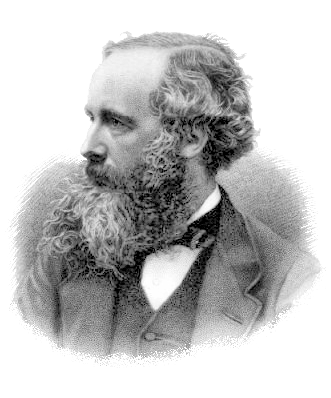
\includegraphics[width=1\textwidth]{Presentacion/James_Clerk_Maxwell.png}
			\end{figure}
			
		\end{columns}
		
		
		
		
		\end{frame}
		
		\begin{frame}
		\frametitle{Campos en medios materiales}
		\centering Si el medio es lineal, isotrópico y homogéneo: %Si anisotrópico, Xe variaría con la dir. Si inhomogéneo, Xe variaría con la posición. Si no lineal, P debería calcularse como una serie de potencias.
		
		\begin{align*}
		\vec{D} = \epsilon_0 \vec{E} + \vec{P}_e = \epsilon_0 (1+\chi_e)\vec{E} = \epsilon \vec{E} &= (\epsilon' - j \epsilon'') \vec{E}\\
		\vec{B} = \mu_0 (\vec{H} + \vec{P}_m) = \mu_0 (1+\chi_m)\vec{H} = \mu \vec{H} &= (\mu' - j \mu'') \vec{H}.
		\end{align*}
		
		\centering Si el material posee una conductividad $\sigma$ independiente del campo eléctrico aplicado, se cumple la Ley de Ohm:
		
		\begin{align*}
		\vec{J} &= \sigma \vec{E} \Rightarrow \vec{D} = \left( \epsilon' - j\epsilon'' - j \frac{\sigma}{\omega} \right) \vec{E}.
		\end{align*}
		
		\begin{block}{\centering Tangente de pérdidas}
			\setlength\abovedisplayskip{0pt}
			\begin{align*}
			\tan \; \delta &= \frac{\omega \epsilon'' + \sigma}{\omega \epsilon'}.
			\end{align*}
		\end{block}
		
		
		\end{frame}
		
		\subsection{Ondas electromagnéticas}
		\begin{frame}
			\frametitle{Ondas electromagnéticas (I)}
			
			\begin{figure}[h]
				\centering
				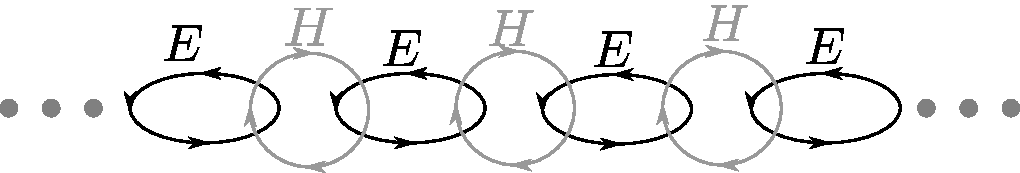
\includegraphics[width=1\textwidth]{Presentacion/onda_em.pdf}
			\end{figure}
			
			\centering En una región libre de fuentes, se pueden deducir las ecuaciones de Helmholtz para ondas monocromáticas, a partir de las ecuaciones de Maxwell.
					
			\begin{align*}
			\left.\begin{array}{rr@{\mskip\thickmuskip}l}
			\nabla^2  \vec{E} + \gamma^2 \vec{E} &= 0\\
			\nabla^2 \vec{H} + \gamma^2 \vec{H}& = 0
			\end{array} \right\}
			\quad \implies \quad
			\left\{\begin{array}{r@{\mskip\thickmuskip}l}
			\vec{E}(x,y,z) &= \vec{E}_0 e^{\pm j \vec{\gamma}\cdot \vec{r}}. \\
			\vec{H}(x,y,z) &= \vec{H}_0 e^{\pm j \vec{\gamma}\cdot \vec{r}}.
			\end{array}\right.
			\end{align*}
			
			\begin{block}{}
				\setlength\abovedisplayskip{0pt}
				\begin{align*}
				\centering
				\gamma &= -j\alpha + \beta = j\omega \sqrt{\mu (\epsilon'-j\epsilon'') - j \sigma \epsilon/\omega}.\\
				\vec{\gamma} &= \vec{\gamma}_x + \vec{\gamma}_y +\vec{\gamma}_z.
				\end{align*}
			\end{block}

		\end{frame}
	
		\begin{frame}
			\frametitle{Ondas electromagnéticas (II)}
			
			Para las ondas planas,
			
			\begin{block}{}
				\setlength\abovedisplayskip{0pt}
				\begin{align*}
				\vec{H}(\vec{r},t) &= \pm \frac{\hat{\beta} \times \vec{E}(\vec{r},t)}{\eta}.
				\end{align*}
			\end{block}
		
		
		
			\begin{columns}[c] % The "c" option specifies centered vertical alignment while the "t" option is used for top vertical alignment
				
				\column{.45\textwidth} % Left column and width
				
				\begin{block}{\centering Impedancia de onda}
					\setlength\abovedisplayskip{0pt}
					\begin{align*}
					\eta &= \frac{j \omega \mu}{\gamma }.
					\end{align*}
				\end{block}
			
				\begin{block}{\centering Velocidad de fase}
					\setlength\abovedisplayskip{0pt}
					\begin{align*}
					v_p &= \omega/\beta = c/\sqrt{\mu_r \epsilon_r}.
					\end{align*}
				\end{block}
			
				
				
				\column{.45\textwidth} % Right column and width
				
				\begin{block}{\centering Prof. penetración}
					\setlength\abovedisplayskip{0pt}
					\begin{align*}
					\label{eq:prof_penetacion}
					\delta_s = -1/\alpha &= \sqrt{\frac{2}{\omega \mu \sigma}}.
					\end{align*}
				\end{block}
			
				\begin{block}{\centering Velocidad de grupo}
					\setlength\abovedisplayskip{0pt}
					\begin{align*}
					v_g &= d\omega/d\beta.
					\end{align*}
				\end{block}
			
			\end{columns}
			
			\begin{block}{\centering Componentes del campo eléctrico que se desplaza en dirección $z$}
				\setlength\abovedisplayskip{0pt}
				\begin{align*}
				E_i(z) = E_i \; e^{-j\gamma z} = E_i \; e^{-\alpha z} \; e^{-j \beta z}, \quad i=x,y.
				\end{align*}
			\end{block}

		\end{frame}
		
		\subsection{Antenas}
		
		\begin{frame}
			\frametitle{Fuentes de ondas electromagnéticas: Antenas}
			\begin{block}{Antena}
				\centering
				Interfaz para las ondas electromagnéticas entre el espacio libre y un dispositivo de guía, generalmente metálico.\\
				\textbf{Objetivo}: Recibir y transmitir energía eficientemente.
			\end{block}
					
			\only<2>{\begin{block}{}
				Se suelen utilizar en conjuntos radiantes, dispuestas geométricamente.\\
				
					-1926: Yagi-Uda.\\
					-Segunda guerra mundial: Conjuntos de antena de fase variable. \\
					-1950: Desfasadores de ferrita, fase completa.
			\end{block}
		
			\begin{figure}[h]
				\centering
				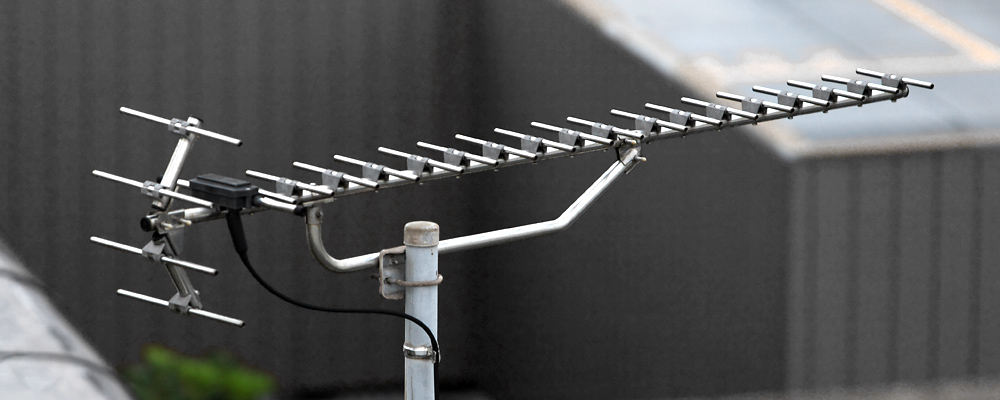
\includegraphics[width=0.5\textwidth]{Presentacion/yagi-uda.JPG}
			\end{figure}}
			
		\end{frame}
		
		\begin{frame}
			\frametitle{Acoplamiento entre antenas}
			\begin{block}{Responsables}
				\begin{itemize}
					\item Acoplamiento espacial entre elementos por onda espacial ($\downarrow \propto 1/\rho$).
					\item Acoplamiento espacial por onda de superficie ($\downarrow \propto 1/\sqrt\rho$).
					\item Acoplamiento por red de alimentación (alimentación no independiente).
				\end{itemize}
			\end{block}
			
			\begin{align*}
			\begin{bmatrix}
			V_1 \\ V_2 \\ \vdots \\ V_N
			\end{bmatrix}
			=
			\underbrace{\begin{bmatrix}
				Z_{11} & Z_{12} & \cdots & Z_{1N} \\
				Z_{12} & Z_{22} & \cdots & Z_{2N} \\
				\vdots & \vdots & \cdots & \vdots \\
				Z_{1N} & Z_{2N} & \cdots & Z_{NN} \\
				\end{bmatrix}}_{Z}
			\begin{bmatrix}
			I_1 \\ I_2 \\ \vdots \\ I_N
			\end{bmatrix}
			\end{align*}
			
		\end{frame}
		
		
		% Comparar Masters Eq con Shrodinger. Modos.
		\subsection{Ondas de superficie}
		
			\begin{frame}
			\frametitle{Ondas de superficie}
			
			\begin{block}{}
				\centering
				Se propagan en un plano.
				
				Comportamiento evanescente en la dirección normal.
			\end{block}
			
			\begin{figure}[]
				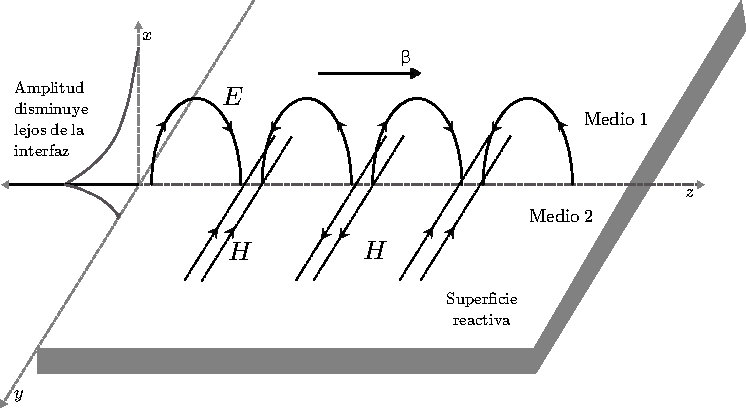
\includegraphics[width=0.65\textwidth]{intro_electro/ondas-superficie-3d.pdf}
			\end{figure}
		
			\begin{columns}[c] % The "c" option specifies centered vertical alignment while the "t" option is used for top vertical alignment
				\column{.55\textwidth}
				\begin{itemize}
					\item Planos conductores.
					\item Planos conductores recubiertos de dieléctrico.
				\end{itemize}
				\column{.51\textwidth}

				\begin{itemize}
					\item Planos corrugados.
					\item Interfaz entre dos medios distintos.
				\end{itemize}
			\end{columns}
			
			\end{frame}
	
			\begin{frame}
			\frametitle{Ondas de Zenneck}
			
			\begin{columns}[c] % The "c" option specifies centered vertical alignment while the "t" option is used for top vertical alignment
				\column{.42\textwidth}
				\begin{itemize}
					\item TM.
					\item Bajas pérdidas.
					\item Ángulo de Brewster: $Z_1 = Z_2$
				\end{itemize}
			
				
				\begin{align*}
				Z_1 = \frac{{E_z}_1}{{H_y}_1} = \eta_0 \cos\; \theta_i = \frac{\gamma_{x_1}}{\gamma_1} \eta_0\\
				Z_2 = \frac{{E_z}_2}{{H_y}_2} = \eta_2 \cos \; \theta_t = \frac{\gamma_{x_2}}{\gamma_2} \eta_2
				\end{align*}
				
				\begin{block}{}
					\centering
				$\gamma$ a uno y otro lado de la interfaz es complejo.
				\end{block}
			
				\column{.6\textwidth}
				
				\begin{figure}
					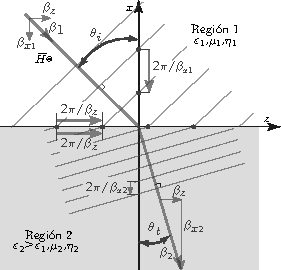
\includegraphics[width=\textwidth]{intro_electro/onda-superficie-incidencia-brewster.pdf}
				\end{figure}
			\end{columns}
			
			\end{frame}
		
			\begin{frame}
			\frametitle{Impedancia de superficie y constante de propagación (TM)}
			
			\centering Si se asume una impedancia de superficie $Z_s = R_s + j X_s$, al igualar la impedancia de onda a la de superficie:
			
			\begin{block}{TM}
			\setlength\abovedisplayskip{0pt}
			\begin{align*}
				\gamma_{x_1} & = \gamma_1 \frac{Z_1}{\eta_0} = \gamma_1 Z_s = \gamma_1 R_s + j \gamma_1 X_s,\\
				\gamma_z &= \beta_z - j\alpha_z =\sqrt{(\gamma_1^2 - \gamma_{x_1}^2)} = \gamma_1 \sqrt{1+X_s^2 - R_s^2 {\color{red}-} 2jR_s X_s}.
			\end{align*}
			\end{block}
		
			\only<1>{
			\begin{columns}[c]
				\column{.48\textwidth}
				\begin{itemize}
					\item $X_s > 0$: Reactancia inductiva:
					\begin{itemize}
						\item $\uparrow \alpha_x$: Decrecimiento exponencial en $x$.\\
						\item $\alpha_z > 0$: Decrecimiento exponencial en $z$.
						\item Menor $v_p$.
					\end{itemize}
				\end{itemize}
			
				\column{.44\textwidth}
				\begin{itemize}
					\item Si $R_s X_s$ es pequeño: Baja atenuación en $z$.
				\end{itemize}
				
				\begin{block}{}
					\centering
					Para ondas de superficie TM:
					\begin{itemize}
						\centering
						\item $\uparrow X_s$ \\
						\item $\downarrow R_s$.
					\end{itemize}
				\end{block}
			\end{columns}
			}
		
			\only<2>{\begin{block}{TE}
				\setlength\abovedisplayskip{0pt}
				\begin{align*}
				\gamma_{x_1} &= -\frac{\gamma_1}{Z_s} = -\gamma_1 \frac{R_s}{{\color{red}R_s^2+X_s^2}}-j\frac{X_s}{{\color{red}R_s^2+X_s^2}},\\
				\gamma_z &= \beta_z-j\alpha_z= \sqrt{(\gamma_1^2 - \gamma_{x_1}^2)} = \frac{\gamma_1}{{\color{red}R_s^2+X_s^2}} \sqrt{1+X_s^2 - R_s^2 {\color{red}+} 2jR_s X_s}.
				\end{align*}
			\end{block}}
	
			\end{frame}
		
			\begin{frame}
				\only<1>{\begin{figure}[htp]
					\centering
					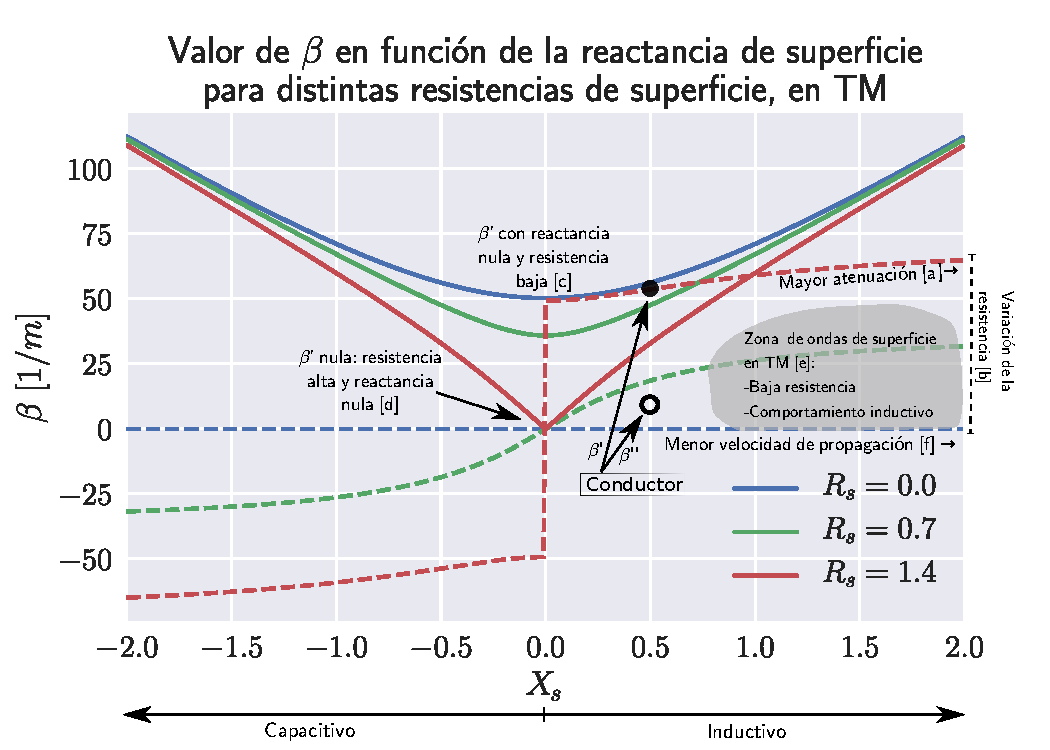
\includegraphics[width=\textwidth]{intro_electro/plot-beta-reactancia-TM.pdf}
				\end{figure}}
			
				\only<2>{\begin{figure}[htp]
					\centering
					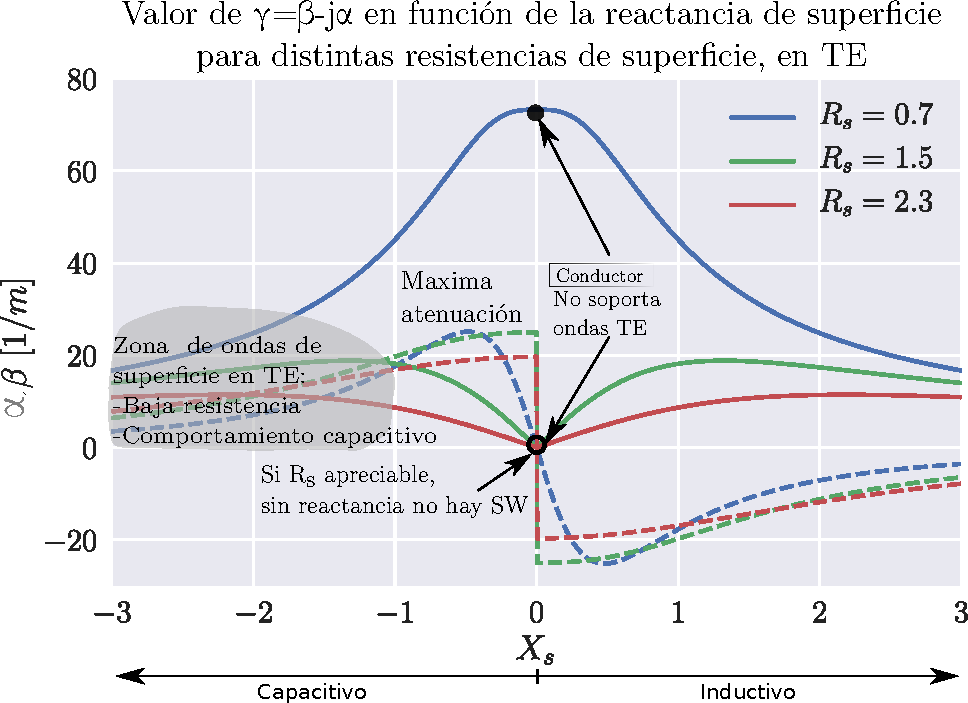
\includegraphics[width=\textwidth]{intro_electro/plot-beta-reactancia-TE.pdf}
				\end{figure}}
			\end{frame}
		
		\begin{frame}
		\frametitle{Condiciones para la propagación sobre un plano conductor}
		
			\begin{block}{\centering Polarización TM}
				\begin{itemize}
					\centering
					\item Comportamiento {\color{red} inductivo}.
					\item Resistividad baja.
				\end{itemize}
			\end{block}
			\begin{block}{\centering Polarización TE}
				\begin{itemize}
					\centering
					\item Comportamiento {\color{red} capacitivo}.
					\item Resistividad baja.
				\end{itemize}
			\end{block}
		
			\centering Para volver más inductiva a la superficie, se puede recubrir al plano conductor con un dieléctrico.
		\end{frame}
	
		\begin{frame}
			\frametitle{Comportamiento para plano de tierra cubierto por un dieléctrico fino}
			\begin{figure}[h]
				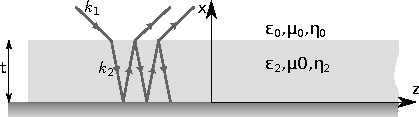
\includegraphics[width=\textwidth]{intro_electro/incidencia-coated-conductor.pdf}
			\end{figure}
		
			\begin{columns}[c]
				\column{.54\textwidth}
				\centering Caso TM:
				
				\begin{align*}
					\begin{cases}
						(\gamma_{x_2} h)^2 + (\alpha_{x_1} h)^2 = (\epsilon_{r_2} - 1) (\gamma_1 h)^2\\
						\gamma_{x_2} h \tan (\gamma_{x_2} h) = |\alpha_{x_1}| \epsilon_{r_2} h.
					\end{cases}
				\end{align*}
				
				\column{.45\textwidth}
				\centering Caso TE:
				
				\begin{align*}
					\begin{cases}
						(\gamma_{x_2} h)^2 + (\alpha_{x_1} h)^2 = (\epsilon_{r_2} - 1) (\gamma_1 h)^2 \\
						\gamma_{x_2} h \cot (\gamma_{x_2} h) = -|\alpha_{x_1}| \epsilon_{r_2} h.
					\end{cases}
				\end{align*}
	
			\end{columns}
		\end{frame}
		
		\begin{frame}
			\begin{columns}[c]
				\column{.52\textwidth}
				\begin{figure}[h]
					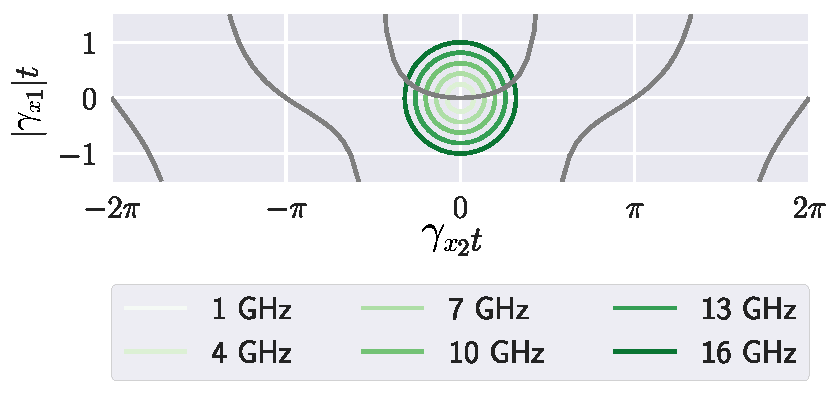
\includegraphics[width=\textwidth]{intro_electro/TM-tan-implicito}
				\end{figure}
				\begin{figure}[h]
					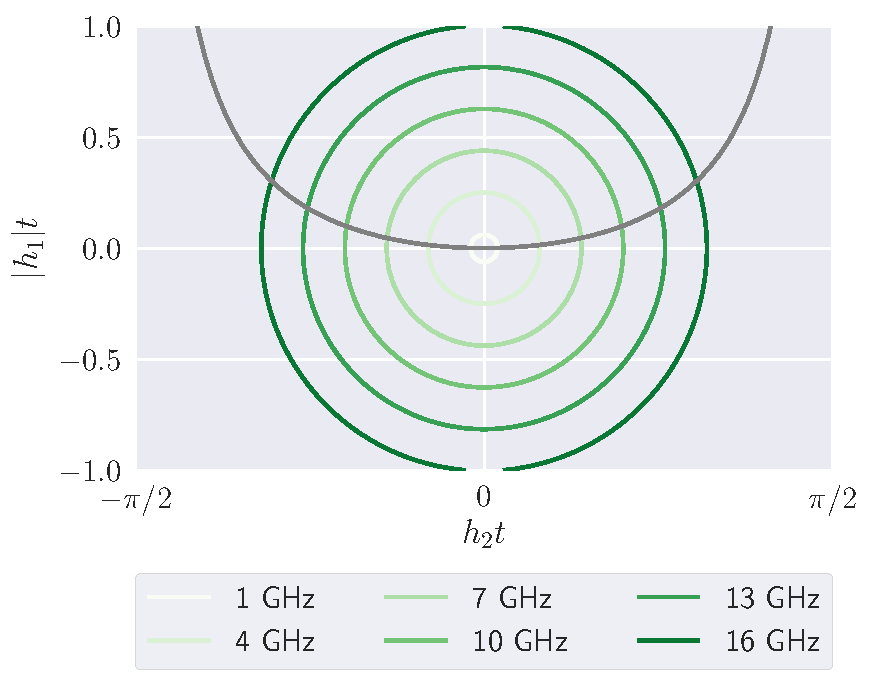
\includegraphics[width=\textwidth]{intro_electro/TM-tan-implicito-zoom}
				\end{figure}
				
				\column{.52\textwidth}
				\begin{figure}[h]
					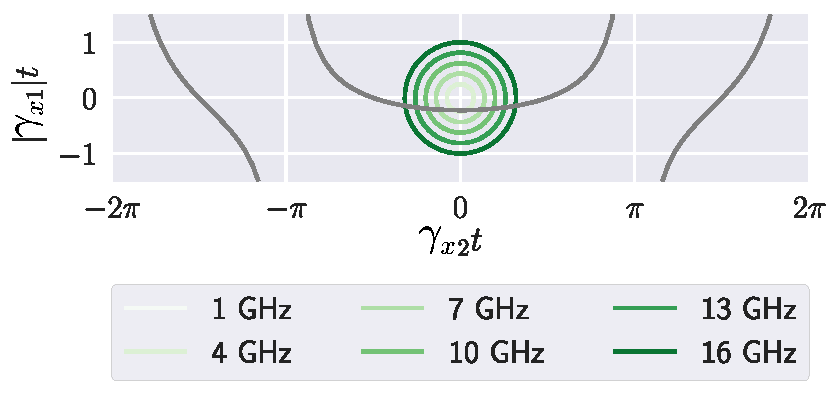
\includegraphics[width=\textwidth]{intro_electro/TE-tan-implicito}
				\end{figure}
				\begin{figure}[h]
					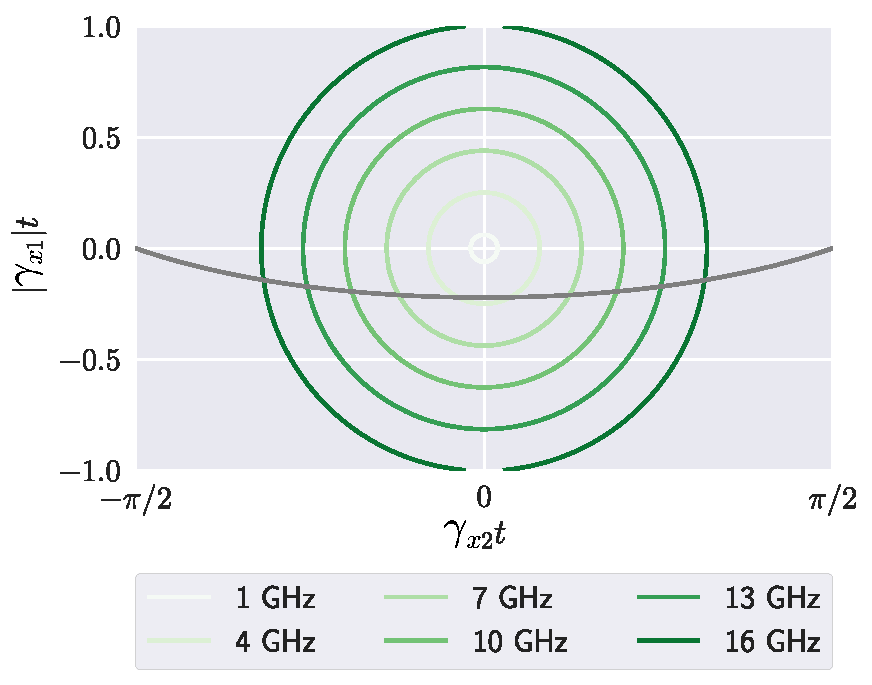
\includegraphics[width=\textwidth]{intro_electro/TE-tan-implicito-zoom}
				\end{figure}
			\end{columns}
		\end{frame}
	
	
		\begin{frame}
			\frametitle{Impedancia de superficie: GND+FR4}
			\begin{align*}
				Z_s^{TM} = j \frac{\cos \theta_t}{\sqrt{\epsilon_{r_2}}}\tan(\gamma_2 h \cos\theta_t) = j \frac{\cos \theta_t}{\sqrt{\epsilon_{r_2}}}\tan(	\omega\sqrt{\epsilon_{r_2} \mu_0 \epsilon_0} h \cos\theta_t)
			\end{align*}
		
			\begin{columns}[c]
				\column{.51\textwidth}
				\begin{figure} [H]
					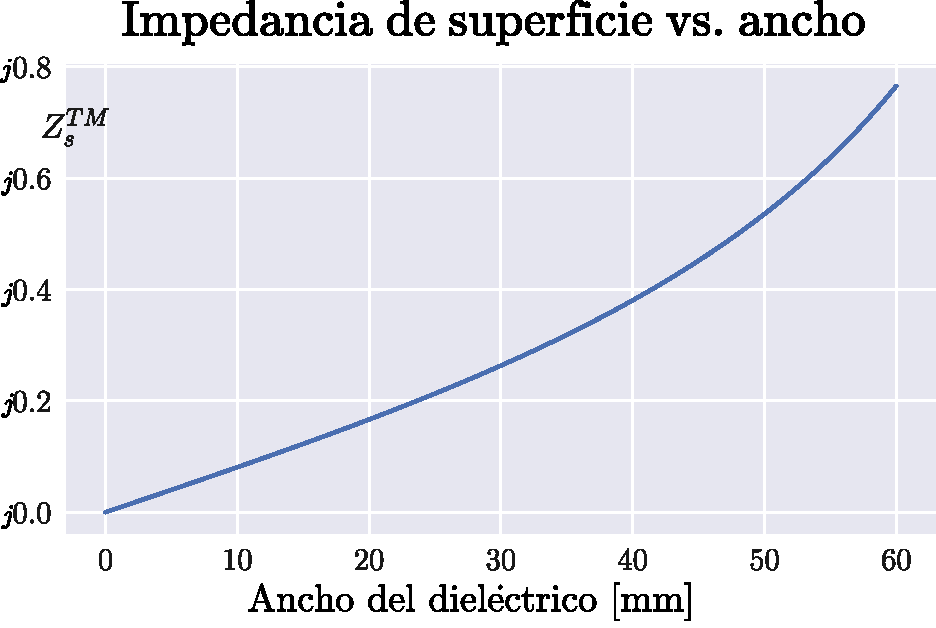
\includegraphics[width=\textwidth]{intro_electro/plot-zstm-funciont2.pdf}
				\end{figure}
				\column{.51\textwidth}
				\begin{figure} [H]
					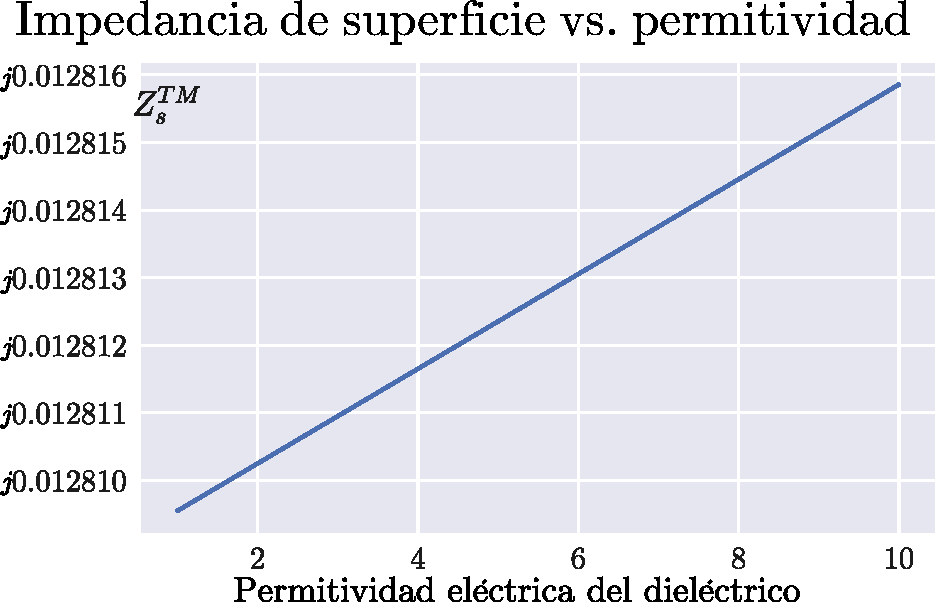
\includegraphics[width=\textwidth]{intro_electro/plot-zstm-funcioner2.pdf}
				\end{figure}
				
			\end{columns}
		\end{frame}
	
		\begin{frame}
			\frametitle{En resúmen}
			\begin{block}{}
				\centering
				No existirán ondas de superficie de polarización TE en el plano de tierra recubierto por 1.6 mm de espesor de FR4, hasta los 25 GHz.
			\end{block}
		
			\begin{block}{}
				\centering
				$\uparrow \text{ancho del sustrato} \Rightarrow\; \uparrow$ ondas de superficie (TM)
			\end{block}
			
			\begin{block}{}
				\centering
				$\uparrow \text{permitividad eléctrica del sustrato} \Rightarrow\; \uparrow$ ondas de superficie (TM)
			\end{block}
		\end{frame}
		
		\subsection{Antenas \textit{microstrip}}
		
		\begin{frame}
			\frametitle{Antenas \textit{microstrip}}
			\begin{columns}
				\column{.45\textwidth} % Right column and width
				\begin{itemize}
					\item Bajo costo, peso y perfil.
					\item Construcción sencilla.
					\item Alto Q (resonantes).
					\item {\color{red}Bajo acoplamiento con elementos cercanos. Campos contenidos en el sustrato.}
				\end{itemize}
				\begin{block}{}
					\centering
					$\uparrow \epsilon_r \Rightarrow \downarrow$ acoplamiento.
				\end{block}			
				\column{.45\textwidth} % Right column and width
				\begin{itemize}
					\item Baja eficiencia.
					\item Baja potencia.
					\item Polarización impura.
					\item {\color{red}Alto acoplamiento con elementos ubicados sobre la superficie.}
				\end{itemize}
				\begin{block}{}
					\centering
					$\uparrow \epsilon_r \Rightarrow \uparrow$ acoplamiento.
				\end{block}	
			\end{columns}
		\end{frame}
	
	
		\begin{frame}
			\frametitle{Modelo de líneas de transmisión}
			\centering Antena rectangular: Dos aperturas radiantes de ancho $W$ y altura $h$, sepadas una distancia $L$ por una línea de trasmisión de impedancia característica conocida $Z_0$.
			
			\begin{figure}[h]
				\centering
				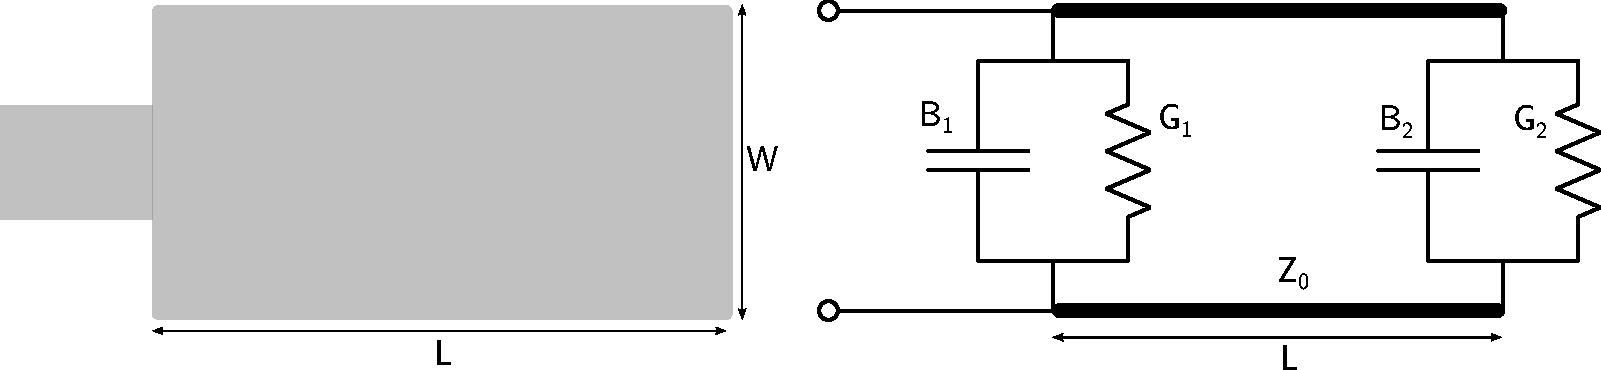
\includegraphics[width=0.9\textwidth]{intro_electro/circuito-equivalente-antena-ms.pdf}
			\end{figure}
		
			\textit{Fringing}: Considerado mediante el uso de una $L_{eff} = L + 2 \Delta L$.
		
		\end{frame}
	
		\begin{frame}
			\frametitle{Modelo de cavidades multimodo}
			\centering Antena rectangular: Cavidad cargada dieléctricamente, limitada por conductores eléctricos en sus caras superior e inferior, y por conductores magnéticos en sus caras laterales.
			
			\begin{align*}
				(f_r)_{nmp} = \frac{1}{2 \pi \sqrt{\mu \epsilon}} \sqrt{\left(\frac{m\pi}{h}\right)^2 + \left(\frac{n\pi}{L}\right)^2 + \left(\frac{p\pi}{W}\right)^2}
			\end{align*}
			
			\begin{figure}[h]
				\centering
				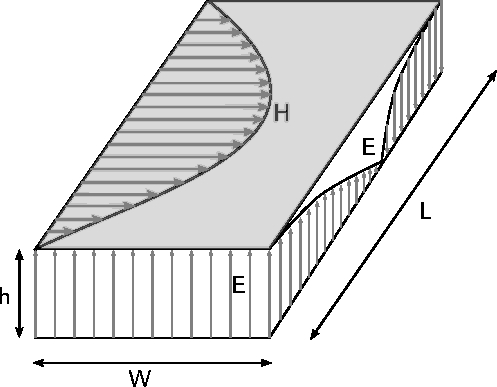
\includegraphics[width=0.49\textwidth]{intro_electro/distribucion-campos-microstrip.pdf}
			\end{figure}
		
		\end{frame}
	
		\begin{frame}
			\frametitle{Acoplamiento mutuo en antenas \textit{microstrip}}
					
			\begin{figure}[h]
				\centering
				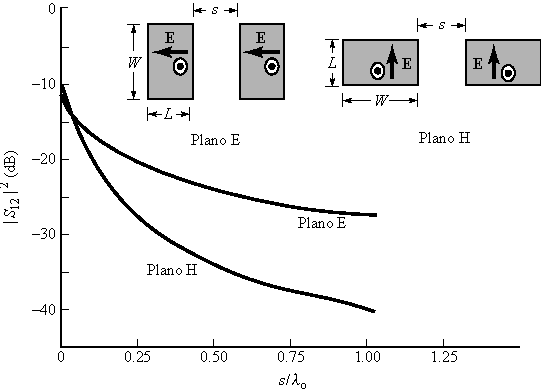
\includegraphics[width=0.9\textwidth]{intro_electro/pozar-acoplamiento.pdf}
			\end{figure}
		
		\end{frame}
		

%------------------------------------------------



\section{Fundamentos de EBGs}
	
	\begin{frame}
	\frametitle{Fundamentos básicos de EBGs}
	\tableofcontents[currentsection,hideothersubsections]
	\end{frame}

	\begin{frame}
		\frametitle{Metamateriales y EBGs}
		\begin{columns}[c]
			\column{.51\textwidth}
			\begin{block}{Metamateriales}
				Estructuras artificiales \textbf{efectivamente homogéneas} para la longitud de onda de interés, que presentan propiedades electromagnéticas que no se encuentran en la naturaleza.
			\end{block}
		
			\begin{block}{EBGs, PBGs, cristales fotónicos}
				Estructuras articiales con capacidades para controlar (en general, atenuar) ondas electromagnéticas a partir de la \textbf{variación periódica} en el espacio de las propiedades del medio respecto de la propagación electromagnética.
			\end{block}
		
			\column{.46\textwidth}
			\begin{figure} [H]
				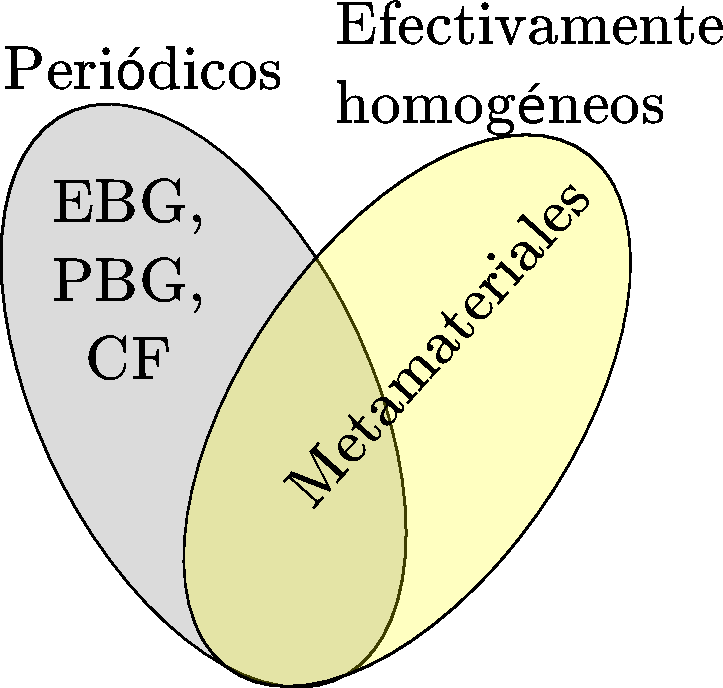
\includegraphics[width=0.9\textwidth]{Presentacion/ebg-metamateriales.pdf}
			\end{figure}
		\end{columns}
	\end{frame}
	
	\begin{frame}
		\frametitle{Reseña histórica}
		\only<1>{
			\begin{columns}[c]
				\column{0.55\textwidth}
				\begin{figure} [H]
					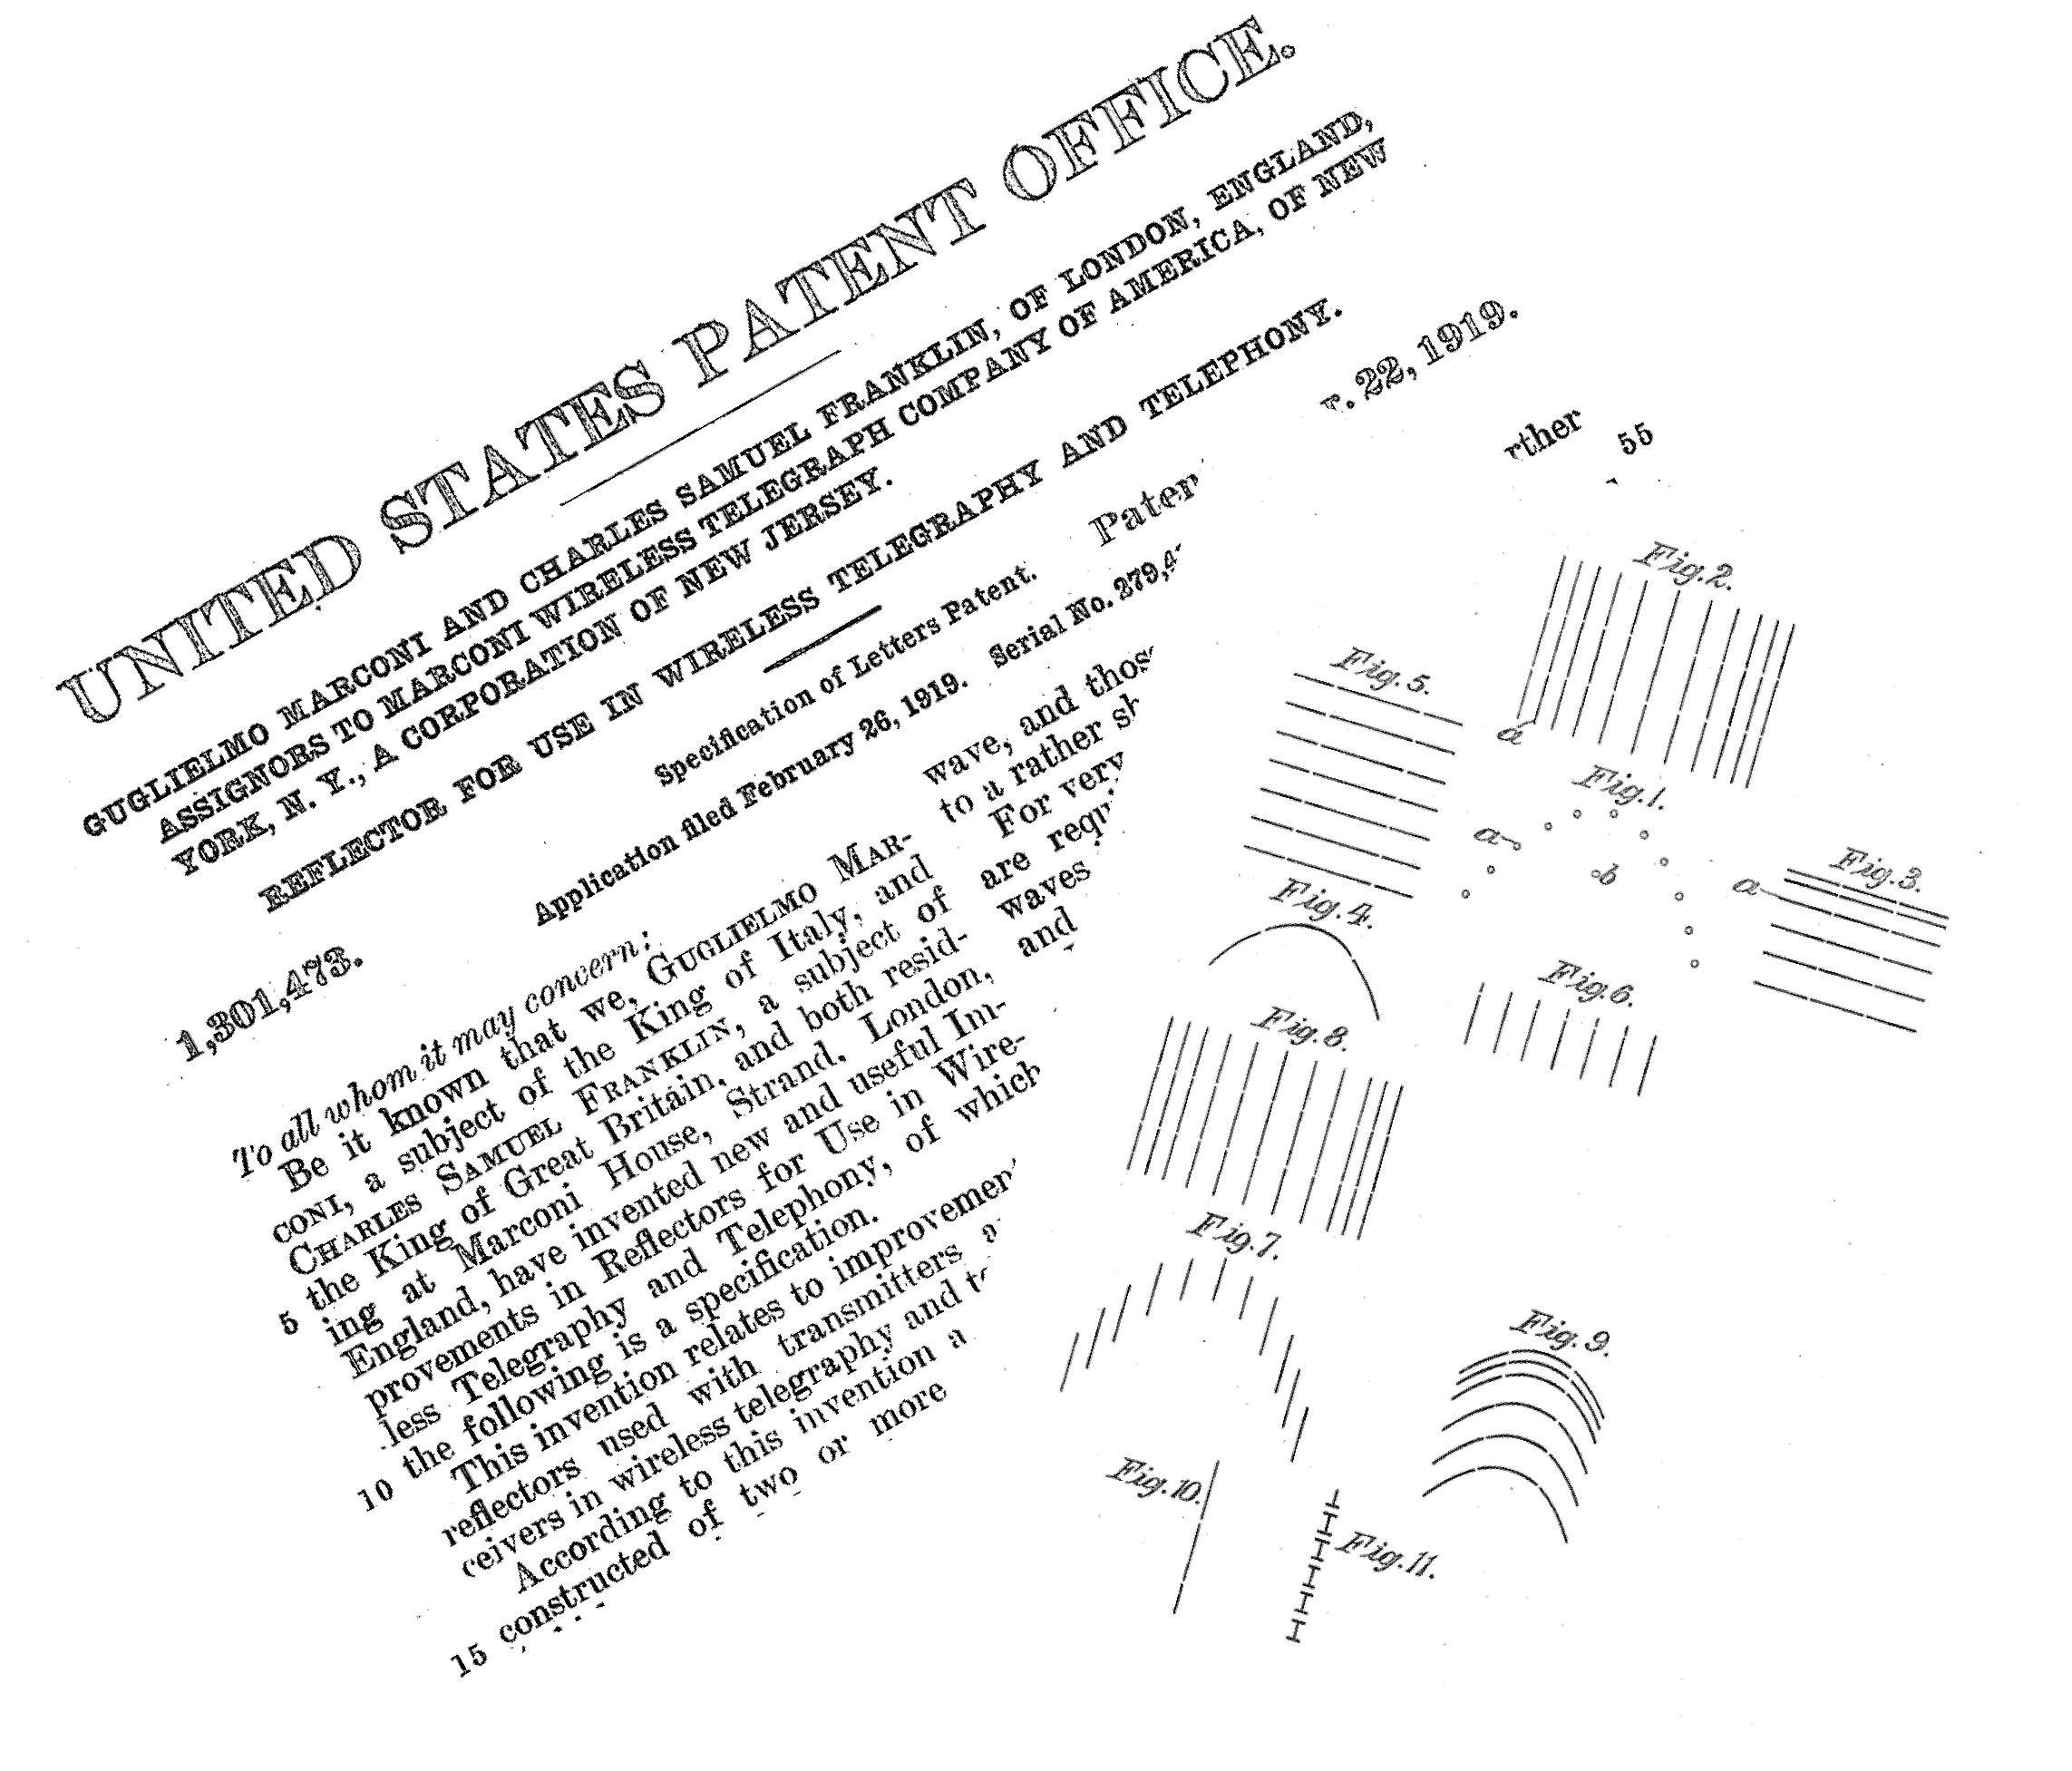
\includegraphics[width=1.2\textwidth]{Presentacion/patenteMarconi.pdf}
				\end{figure}
			
				\column{0.46\textwidth}
				\begin{itemize}
					\item Fines del siglo XVIII: \textbf{Rittenhouse} observó que algunos colores desaparecían cuando se veía luz a través de un pañuelo.
					\item 1919: Guglielmo \textbf{Marconi}, Charles Samuel \textbf{Franklin}: Conductores horizontales como superficie reflectiva para cierta frecuencia (¿Primer FSS?)
				\end{itemize}
			\end{columns}
		}
	
		
		\only<2>{
			\begin{itemize}
				\item 1946: Louis \textbf{Brillouin}: \textit{Wave propagacion in periodic structures: Electric filters and crystal lattices}. Restricciones a los vectores de onda $\gamma$ en un medio periódico.
				\item 1968: Viktor \textbf{Veselago}: Descripción teórica de LHS, velocidad de grupo antiparalela a la velocidad de fase.
			\end{itemize}
		
			\begin{figure}[h]
				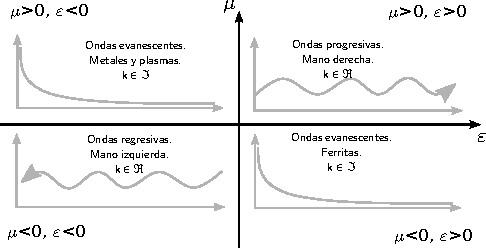
\includegraphics[width=0.8\textwidth]{Fundamentos/OndasSegunEyU.pdf}
			\end{figure}
		}
		
		\only<3>{
			\begin{figure}[htp]
				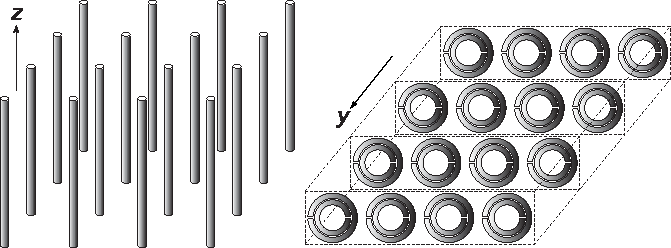
\includegraphics[width=0.8\textwidth]{Fundamentos/pendry.pdf}
			\end{figure}
			
			\begin{itemize}
				\item 1990: \textbf{Smith}: Split Ring Resonators en base a los trabajos de Pendry. Se construyó en 2000.
				\item 1990: \textbf{Ho, Chan, Soukulis}: Conjunto periódico de esferas dieléctricas. Banda prohibida.
				\item 1990: \textbf{Yablonovitch}. Estructura cristalina. Agujeros cilíndricos.
			\end{itemize}
		}
		
		\only<4>{
			\begin{figure}[htp]
				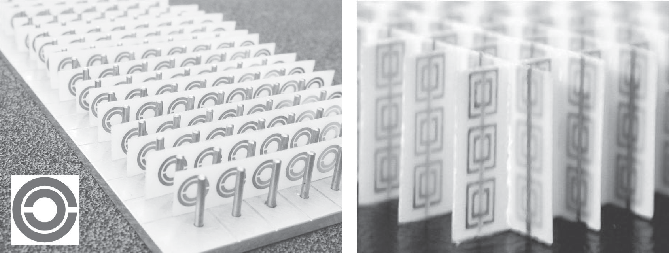
\includegraphics[width=\textwidth]{Fundamentos/metamateriales-smith.pdf}
			\end{figure}
		}
	

		\only<5>{
		\begin{itemize}
			\item 1999: \textbf{Sievenpiper}: HIS. Mushrooms. AMC + EBG.
			\item 2001: \textbf{Yang}: Uniplanar EBG (¿FSS o EBG?)
		\end{itemize}
		
		\begin{columns}[c]
			\column{.51\textwidth}
			\begin{figure}
				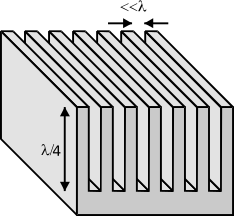
\includegraphics[width=0.8\textwidth]{Fundamentos/superficie-coarrugada.png}
			\end{figure}
		
			\column{.51\textwidth}
			\begin{figure}
				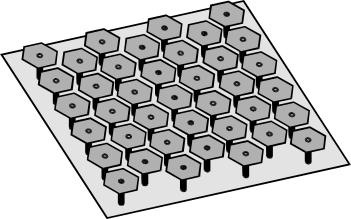
\includegraphics[width=\textwidth]{Fundamentos/sievenpiper.png}
			\end{figure}
		\end{columns}
		}
	\end{frame}
	
	\subsection{Bragg, Bloch-Floquet y espacio recíproco}
	
		\begin{frame}
			\frametitle{Difracción de Bragg}
		
			\begin{figure}[htp]
				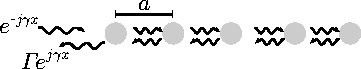
\includegraphics[width=0.6\textwidth]{Fundamentos/bragg1.pdf}
			\end{figure}
			
			\begin{align*}
			\Gamma_t = \Gamma e^{-j\gamma x} + \Gamma e^{-2j\gamma a} e^{-j\gamma x} + \Gamma e^{-4j\gamma a} e^{-j\gamma x} + ... = \Gamma e^{-j\gamma x} \frac{1}{1-e^{-2j\gamma a}},
			\end{align*}
			
			\centering Si $e^{-2j\gamma a} = 1$, la expresión diverge.
			
			 \begin{block}{\centering Condición de Bragg}
			 	\centering
			 	$\gamma = n\pi/a$
			 \end{block}
			% Se podría dar la expresión más general en las diapositivas anexas.
		\end{frame}
	
		\begin{frame}
		\frametitle{Teorema de Bloch y armónicos espaciales}
		\end{frame}
	
		\begin{frame}
		\frametitle{Espacio recíproco}
		\end{frame}
	
	\subsection{Dispersión}
	
		\begin{frame}
		\frametitle{Dispersión en materiales comunes}
		\end{frame}
	
		\begin{frame}
		\frametitle{Representación de la dispersión en 2D}
		\end{frame}
	
		\begin{frame}
		\frametitle{Bandgap electromagnético}
		% Rods, TM, TE, combinación de los dos (Yablo), uso en waveguides. Dibujitos, senos deformes.
		\end{frame}
%------------------------------------------------

\begin{frame}
\frametitle{Table}
\begin{table}
\begin{tabular}{l l l}
\toprule
\textbf{Treatments} & \textbf{Response 1} & \textbf{Response 2}\\
\midrule
Treatment 1 & 0.0003262 & 0.562 \\
Treatment 2 & 0.0015681 & 0.910 \\
Treatment 3 & 0.0009271 & 0.296 \\
\bottomrule
\end{tabular}
\caption{Table caption}
\end{table}
\end{frame}

%------------------------------------------------

\begin{frame}
\frametitle{Theorem}
\begin{theorem}[Mass--energy equivalence]
$E = mc^2$
\end{theorem}
\end{frame}

%------------------------------------------------

\begin{frame}[fragile] % Need to use the fragile option when verbatim is used in the slide
\frametitle{Verbatim}
\begin{example}[Theorem Slide Code]
\begin{verbatim}
\begin{frame}
\frametitle{Theorem}
\begin{theorem}[Mass--energy equivalence]
$E = mc^2$
\end{theorem}
\end{frame}\end{verbatim}
\end{example}
\end{frame}

%------------------------------------------------

\begin{frame}
\frametitle{Figure}
Uncomment the code on this slide to include your own image from the same directory as the template .TeX file.
%\begin{figure}
%\includegraphics[width=0.8\linewidth]{test}
%\end{figure}
\end{frame}

%------------------------------------------------

\begin{frame}[fragile] % Need to use the fragile option when verbatim is used in the slide
\frametitle{Citation}
An example of the \verb|\cite| command to cite within the presentation:\\~

This statement requires citation \cite{p1}.
\end{frame}

%------------------------------------------------

\begin{frame}
\frametitle{References}
\footnotesize{
\begin{thebibliography}{99} % Beamer does not support BibTeX so references must be inserted manually as below
\bibitem[Smith, 2012]{p1} John Smith (2012)
\newblock Title of the publication
\newblock \emph{Journal Name} 12(3), 45 -- 678.
\end{thebibliography}
}
\end{frame}

%------------------------------------------------

\begin{frame}
\Huge{\centerline{The End}}
\end{frame}

%----------------------------------------------------------------------------------------

\section{Modelado}

	\subsection{Ecuación de dispersión}
		\begin{frame} % Need to use the fragile option when verbatim is used in the slide
		\frametitle{Ecuación de dispersión partir de una línea de transmisión}
		\end{frame}
	 
	 	\begin{frame} % Need to use the fragile option when verbatim is used in the slide
	 	\frametitle{Diagrama de dispersión}
 	    \end{frame}
      
     \subsection{Métodos numéricos}
	    \begin{frame} % Need to use the fragile option when verbatim is used in the slide
	    \frametitle{Métodos numéricos}
	 	\end{frame}
	
		\begin{frame} % Need to use the fragile option when verbatim is used in the slide
		\frametitle{Resultados de simulaciones para celda sencilla}
		\end{frame}
		
		\begin{frame} % Need to use the fragile option when verbatim is used in the slide
		\frametitle{Análisis de diagrama de dispersión típico}
		\end{frame}
		
	 \subsection{Análisis paramétrico de una celda sencilla}
	 
	 	\begin{frame} % Need to use the fragile option when verbatim is used in the slide
	 	\frametitle{Variación del ancho del puente}
 		\end{frame}
 	
	 	\begin{frame} % Need to use the fragile option when verbatim is used in the slide
	 	\frametitle{Variación del tamaño de la celda unitaria}
	 	\end{frame}
 	
	 	\begin{frame} % Need to use the fragile option when verbatim is used in the slide
	 	\frametitle{Variación del lado del parche}
	 	\end{frame}
 	
	 	\begin{frame} % Need to use the fragile option when verbatim is used in the slide
	 	\frametitle{Variación del ancho del sustrato}
	 	\end{frame}
 	
\section{Análisis y modelado de la celda de Yang}
		
		\begin{frame} % Need to use the fragile option when verbatim is used in the slide
		\frametitle{Celda de Yang}
		\end{frame}
	
		\begin{frame} % Need to use the fragile option when verbatim is used in the slide
		\frametitle{Comportamiento}
		\end{frame}
	
	\subsection{Construcción del modelo circuital}
		\begin{frame} % Need to use the fragile option when verbatim is used in the slide
		\frametitle{Modelo I}
		\end{frame}
	
		\begin{frame} % Need to use the fragile option when verbatim is used in the slide
		\frametitle{Modelo I: Resultados}
		\end{frame}
	
		\begin{frame} % Need to use the fragile option when verbatim is used in the slide
		\frametitle{Modelo II}
		\end{frame}

		\begin{frame} % Need to use the fragile option when verbatim is used in the slide
		\frametitle{Modelo II: Resultados}
		\end{frame}
		
		\begin{frame} % Need to use the fragile option when verbatim is used in the slide
		\frametitle{Modelo II: Diagrama de dispersión}
		\end{frame}
	
		\begin{frame} % Need to use the fragile option when verbatim is used in the slide
		\frametitle{Modelo III}
		\end{frame}
	
		\begin{frame} % Need to use the fragile option when verbatim is used in the slide
		\frametitle{Modelo III: Resultados}
		\end{frame}
	
		\begin{frame} % Need to use the fragile option when verbatim is used in the slide
		\frametitle{Modelo III: Diagrama de dispersión}
		\end{frame}
	
	\subsection{Comportamiento II}
		\begin{frame} % Need to use the fragile option when verbatim is used in the slide
		\frametitle{Comportamiento de una fila}
		\end{frame}
	
		\begin{frame} % Need to use the fragile option when verbatim is used in the slide
		\frametitle{Comportamiento de una estructura}
		\end{frame}
	
\section{Construcción del algoritmo de simulación en el dominio del tiempo}
		\begin{frame} % Need to use the fragile option when verbatim is used in the slide
		\frametitle{Definiciones}
		\end{frame}
	
		\begin{frame} % Need to use the fragile option when verbatim is used in the slide
		\frametitle{Resultados}
		\end{frame}

\end{document}